\section{Connectionist Temporal Classification}

Consider speech recognition. We have a dataset of audio clips and corresponding
transcripts. Unfortunately, we do not know how the characters in the transcript
align to the audio. This makes training a speech recognizer harder than it
might at first seem.

Without this alignment, the simple approaches are not available to us. We could
devise a rule like ``one character corresponds to ten inputs". But people's
rates of speech vary, so this type of rule can always be broken.  Another
alternative is to hand-align each character to its location in the audio. From
a modeling standpoint this works well -- we would know the ground truth for
each input time-step. However, for any reasonably sized dataset this is
prohibitively time consuming.

This problem is not specific to speech recognition. We see it in many other
places. Handwriting recognition from images or sequences of pen strokes is one
example. Action labelling in videos is another.

\begin{figure}
\centering
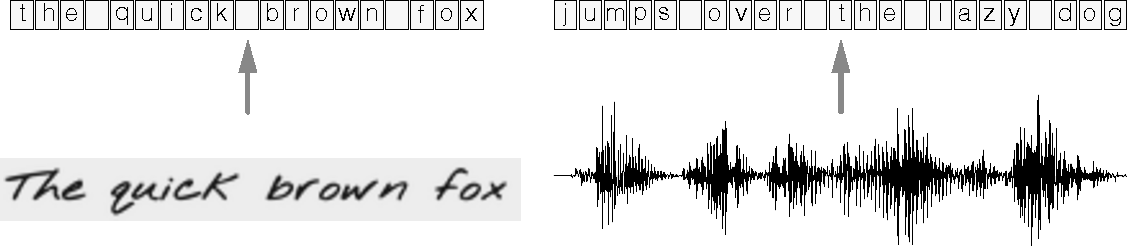
\includegraphics[width=\textwidth]{background/figures/asr_hrr.pdf}
\caption{An example of two sequence transcription problems: handwriting
    recognition (left) and speech recognition (right).}
\label{fig:bg:asr_hrr} 
\end{figure}

Connectionist Temporal Classification (CTC) is a way to get around not knowing
the alignment between the input and the output. As we will see, it is
especially well suited to applications like speech and handwriting recognition.

To be a bit more formal, consider mapping input sequences $X = [x_1, x_2,
\ldots, x_T]$, such as audio, to corresponding output sequences $Y = [y_1, y_2,
\ldots, y_U]$, such as transcripts.  We want to find an accurate mapping from
$X$'s to $Y$'s.

There are challenges which get in the way of us using simpler supervised
learning algorithms. In particular:
\begin{itemize}
  \item Both $X$ and $Y$ can vary in length.
  \item The ratio of the lengths of $X$ and $Y$ can vary.
  \item We don't have an accurate alignment (correspondence of the elements) of
  $X$ and $Y$.
\end{itemize}

The CTC algorithm overcomes these challenges. For a given $X$ it gives us an
output distribution over all possible $Y$'s. We can use this distribution
either to {\it infer} a likely output or to assess the {\it probability} of a
given output.

Not all ways of computing the loss function and performing inference are
tractable. We will require that CTC do both of these efficiently.

{\bf Loss Function:} For a given input, we would like to train our model to
maximize the probability it assigns to the right answer. To do this, we will
need to efficiently compute the conditional probability $p(Y \mid X)$. The
function $p(Y \mid X)$ should also be differentiable, so we can use gradient
descent.

{\bf Inference:} Naturally, after training the model, we want to use it to
infer a likely $Y$ given an $X$.  This means solving
\[
  Y^* \enspace =\enspace \argmax_Y \enspace p(Y \mid X).
\]
Ideally $Y^*$ can be found efficiently. With CTC we will settle for an
approximate solution that is not too expensive to find.

The CTC algorithm can assign a probability for any $Y$ given an $X$. The key to
computing this probability is how CTC thinks about alignments between inputs
and outputs. We will start by looking at these alignments and then show how to
use them to compute the loss function and perform inference.

\subsection{Alignment}

The CTC algorithm is {\it alignment-free} -- it does not require an alignment
between the input and the output. However, to get the probability of an output
given an input, CTC works by summing over the probability of all possible
alignments between the two. We need to understand what these alignments are in
order to understand how the loss function is ultimately calculated.

To motivate the specific form of the CTC alignments, first consider a naive
approach. As an example, assume the input has length six and $Y = \textrm{[c,
a, t]}$. One way to align $X$ and $Y$ is to assign an output character to each
input step and collapse repeats.

\begin{center}
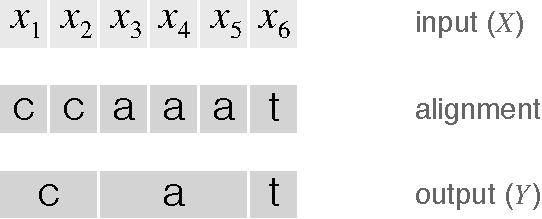
\includegraphics[width=0.5\textwidth]{background/figures/naive_alignment.pdf}
\end{center}

This approach has two problems.
\begin{itemize}
\item Often, it does not make sense to force every input step to align to some
output. In speech recognition, for example, the input can have stretches of
silence with no corresponding output.
\item We have no way to produce outputs with multiple characters in a row.
Consider the alignment [h, h, e, l, l, l, o]. Collapsing repeats will produce
``helo" instead of ``hello".
\end{itemize}

To get around these problems, CTC introduces a new token to the set of allowed
outputs. This new token is sometimes called the {\it blank} token. We refer to
it here as $\epsilon$. The $\epsilon$ token does not correspond to anything and
is simply removed from the output.

The alignments allowed by CTC are the same length as the input. We allow any
alignment which maps to $Y$ after merging repeats and removing $\epsilon$
tokens:

\begin{center}
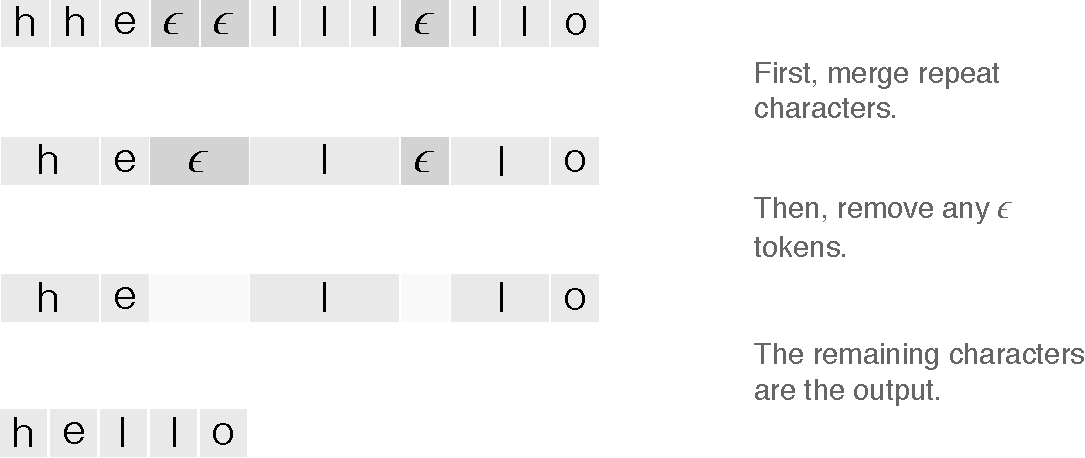
\includegraphics[width=0.7\textwidth]{background/figures/alignment_steps.pdf}
\end{center}

If $Y$ has two of the same character in a row, then a valid alignment must have
an $\epsilon$ between them. With this rule in place, we can differentiate
between alignments which collapse to ``hello" and those which collapse to
``helo".

Let's go back to the output [c, a, t] with an input of length six. Here are
a few more examples of valid and invalid alignments.

\begin{center}
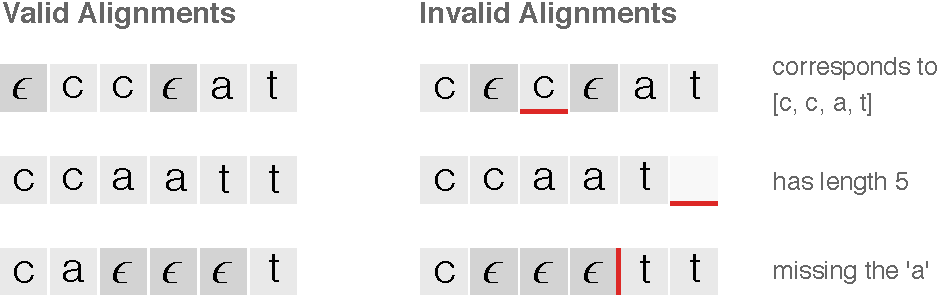
\includegraphics[width=0.7\textwidth]{background/figures/valid_invalid_alignments.pdf}
\end{center}

The CTC alignments have a few notable properties. First, the allowed alignments
between $X$ and $Y$ are monotonic.  If we advance to the next input, we can
keep the corresponding output the same or advance to the next one. A second
property is that the alignment of $X$ to $Y$ is many-to-one. One or more input
elements can align to a single output element but not vice-versa. This implies
a third property: the length of $Y$ cannot be greater than the length of $X$.

\subsection{Loss Function}

The CTC alignments give us a natural way to go from probabilities at each
time-step to the probability of an output sequence. To be precise, the CTC
objective for a single $(X, Y)$ pair is:
\begin{align*}
p(Y \mid X) \;\; = \sum_{A \in \mathcal{A}_{X,Y}}
      \prod_{t=1}^T \; p_t(a_t \mid X)
\end{align*}
The CTC conditional probability marginalizes over the set of valid alignments
computing the probability for a single alignment step-by-step.

Models trained with CTC typically use a recurrent neural network (RNN) to
estimate the per time-step probabilities, $p_t(a_t \mid X)$. An RNN usually
works well since it accounts for context in the input, but we're free to use
any learning algorithm which produces a distribution over output classes given
a fixed-size slice of the input.

If we are not careful, the CTC loss can be very expensive to compute. We could
try the straightforward approach and compute the score for each alignment
summing them all up as we go. The problem is there can be a massive number of
alignments.\footnote{For a $Y$ of length $U$ without any repeat characters and
an $X$ of length $T$ the size of the set is ${T + U \choose T - U}$. For
$T=100$ and $U=50$ this number is almost $10^{40}$.} For most problems this
would be too slow.

Thankfully, we can compute the loss much faster with a dynamic programming
algorithm. The key insight is that if two alignments have reached the same
output at the same step, then we can merge them.

Since we can have an $\epsilon$ before or after any token in $Y$, it is easier
to describe the algorithm using a sequence which includes them. We will work
with the sequence
\[
Z \enspace =\enspace [\epsilon, ~y_1, ~\epsilon, ~y_2,~ \ldots, ~\epsilon, ~y_U, ~\epsilon]
\]
which is $Y$ with an $\epsilon$ at the beginning, end, and between every
character.

Let $\alpha$ be the score of the merged alignments at a given node. More
precisely, $\alpha_{s, t}$ is the CTC score of the subsequence $Z_{1:s}$ after
$t$ input steps.  The final CTC score, $P(Y \mid X)$, is computed from from the
$\alpha$'s at the last time-step. As long as we know the values of $\alpha$ at
the previous time-step, we can compute $\alpha_{s, t}$. There are two cases.

\begin{figure}[ht!]
\centering
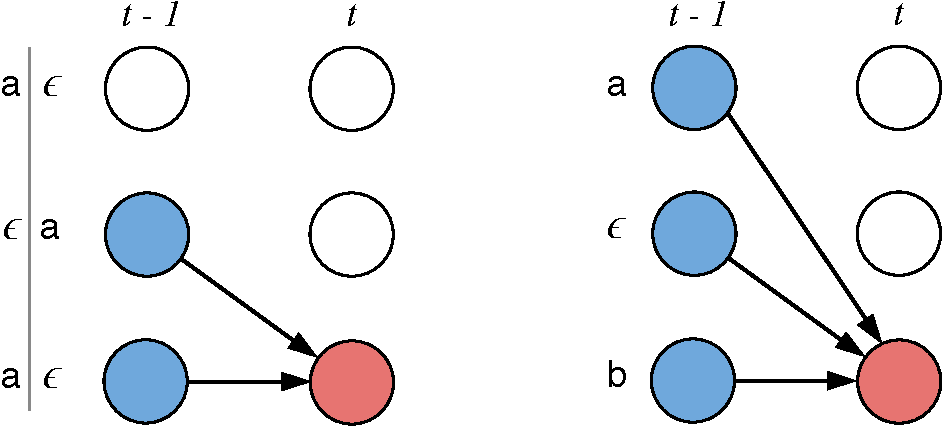
\includegraphics[width=0.5\textwidth]{background/figures/cases.pdf}
\caption{In Case 1 (left) we cannot skip the previous token whereas Case 2
    (right) we can.}
\end{figure}

{\bf Case 1:} In this case, we cannot jump over $z_{s-1}$, the previous token
in $Z$. The first reason is that the previous token can be an element of $Y$,
and we cannot skip elements of $Y$. Since every element of $Y$ in $Z$ is
followed by an $\epsilon$, we can identify this when $z_{s} = \epsilon$. The
second reason is that we must have an $\epsilon$ between repeat characters in
$Y$. We can identify this when $z_s = z_{s-2}$.

To ensure we do not skip $z_{s-1}$, we can either be there at the previous
time-step or have already passed through at some earlier time-step. As a result
there are two positions we can transition from.
\begin{align*}
\alpha_{s, t} \; = \; (\alpha_{s-1, t-1} + \alpha_{s, t-1}) \cdot p_t(z_{s} \mid X)
\end{align*}
In words, the probability of the subsequence $Z_{1:s}$ after $t$ input steps is
the sum of the probabilities of the two valid subsequences after $t-1$ input
steps times the probability of the current character at input step $t$.

{\bf Case 2:} In the second case, we are allowed to skip the previous token in
$Z$. We have this case whenever $z_{s-1}$ is an $\epsilon$ between unique
characters. As a result there are three positions we could have come from at
the previous step.
\begin{align*}
\alpha_{s, t} \; = \; (\alpha_{s-2, t-1} + \alpha_{s-1, t-1} + \alpha_{s, t-1}) \cdot
    p_t(z_{s} \mid X).
\end{align*}

\begin{figure}
\centering
    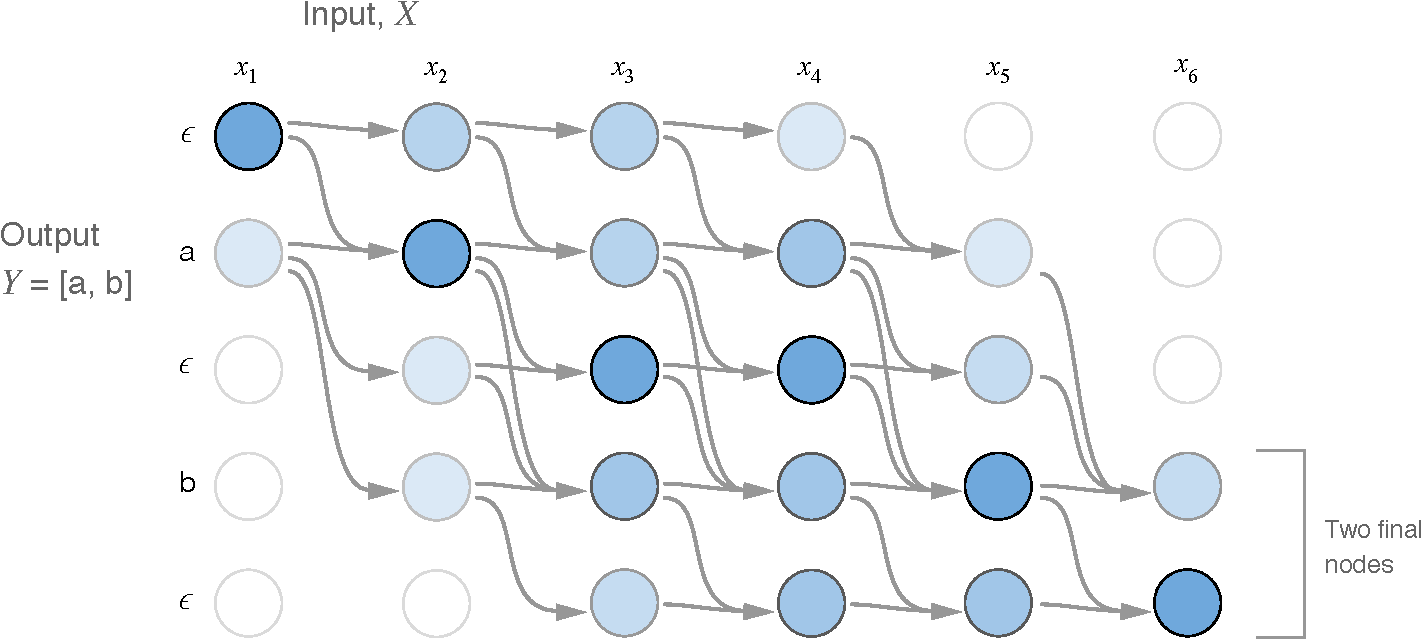
\includegraphics[width=\textwidth]{background/figures/ctc_cost.pdf}
\caption{An example of the computation performed by the dynamic programming
    algorithm. Every valid alignment has a path in this graph. Node $(s, t)$ in
    the diagram represents $\alpha_{s, t}$ – the CTC score of the subsequence
    $Z_{1:s}$ after $t$ input steps.}
\end{figure}

There are two valid starting nodes and two valid final nodes since the
$\epsilon$ at the beginning and end of the sequence is optional. The complete
probability is the sum of the two final nodes.

Now that we can efficiently compute the loss function, the next step is to
compute a gradient and train the model. The CTC loss function is differentiable
with respect to the per time-step output probabilities since it's just sums and
products of them. Given this, we can analytically compute the gradient of the
loss function with respect to the (unnormalized) output probabilities and from
there run backpropagation as usual.

For a training set $\mathcal{D}$, the model's parameters are tuned to minimize
the negative log-likelihood
\[
\sum_{(X, Y) \in \mathcal{D}} -\log\; p(Y \mid X)
\]
instead of maximizing the likelihood directly.

\subsection{Inference}

After training the model, we would like to use it to find a likely output for a
given input. More precisely, we need to solve:
\[
Y^* \enspace = \enspace \argmax_Y \enspace p(Y \mid X)
\]
One heuristic is to take the most likely output at each time-step. This gives
us the alignment with the highest probability:
\[
A^* \enspace = \enspace \argmax_A \enspace  \prod_{t=1}^{T} \; p_t(a_t \mid X)
\]
We can then collapse repeats and remove $\epsilon$ tokens to get $Y$.

For many applications this heuristic works well, especially when most of the
probability mass is alloted to a single alignment. However, this approach can
sometimes miss easy to find outputs with much higher probability. The problem
is, it does not take into account the fact that a single output can have many
alignments.

As an example, assume the alignments [a, a, $\epsilon$] and [a, a, a]
individually have lower probability than [b, b, b]. But the sum of their
probabilities is actually greater than that of [b, b, b]. The naive heuristic
will incorrectly propose $Y =$ [b] as the most likely hypothesis. It should
have chosen $Y =$ [a].  To fix this, the algorithm needs to account for the
fact that [a, a, a] and [a, a, $\epsilon$] collapse to the same output.

We can use a modified beam search to solve this. Given limited computation, the
modified beam search will not necessarily find the most likely $Y$. It does, at
least, have the nice property that we can trade-off more computation (a larger
beam-size) for an asymptotically better solution.

A regular beam search computes a new set of hypotheses at each input step. The
new set of hypotheses is generated from the previous set by extending each
hypothesis with all possible output characters and keeping only the top
candidates.

\begin{figure}
\centering
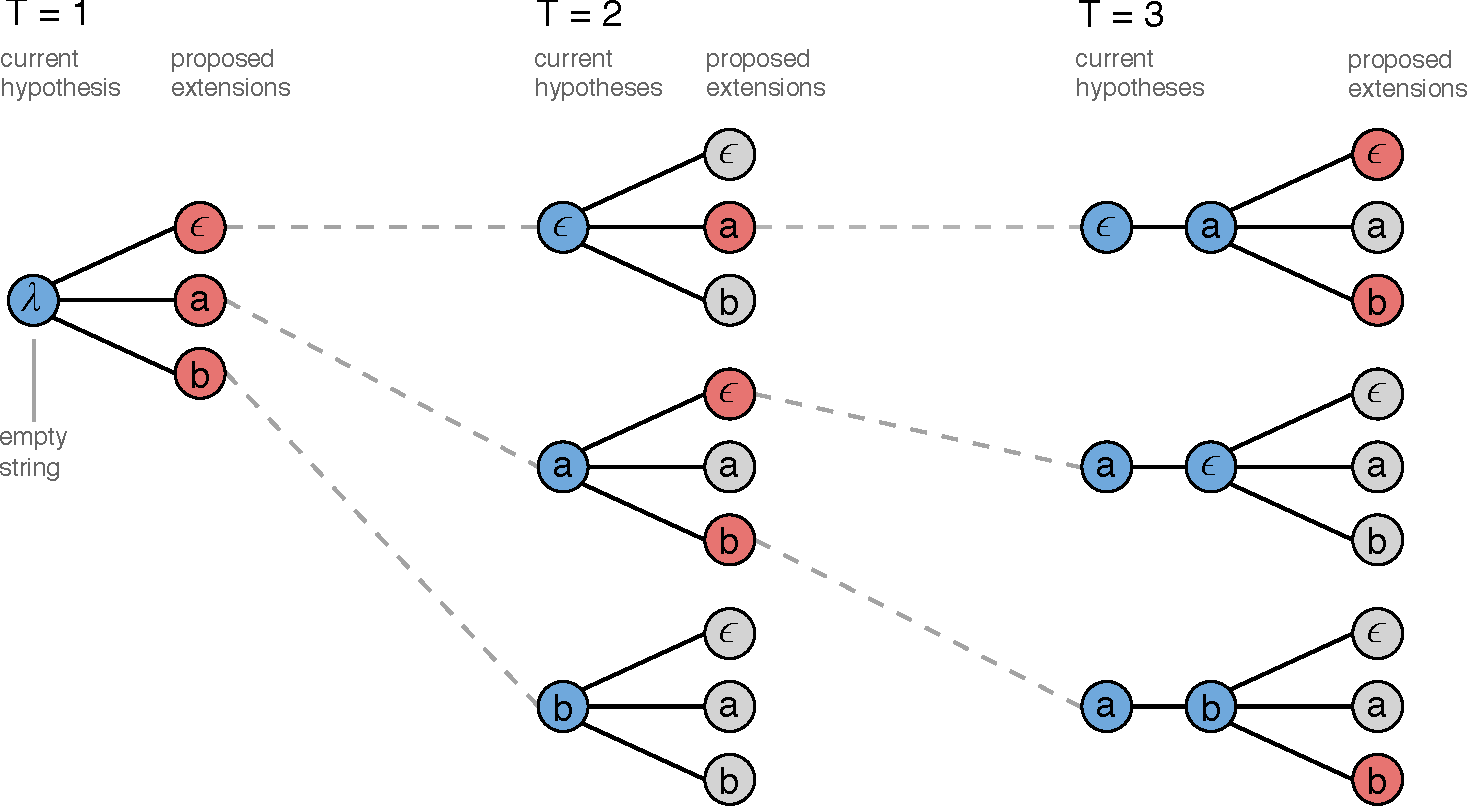
\includegraphics[width=0.8\textwidth]{background/figures/beam_search.pdf}
\caption{A standard beam search algorithm with an alphabet of $\{\epsilon, a,
    b\}$ and a beam size of three.}
\end{figure}

We can modify the vanilla beam search to handle multiple alignments mapping to
the same output. In this case instead of keeping a list of alignments in the
beam, we store the output prefixes after collapsing repeats and removing
$\epsilon$ characters. At each step of the search we accumulate scores for a
given prefix based on all the alignments which map to it.

\begin{figure}
\centering
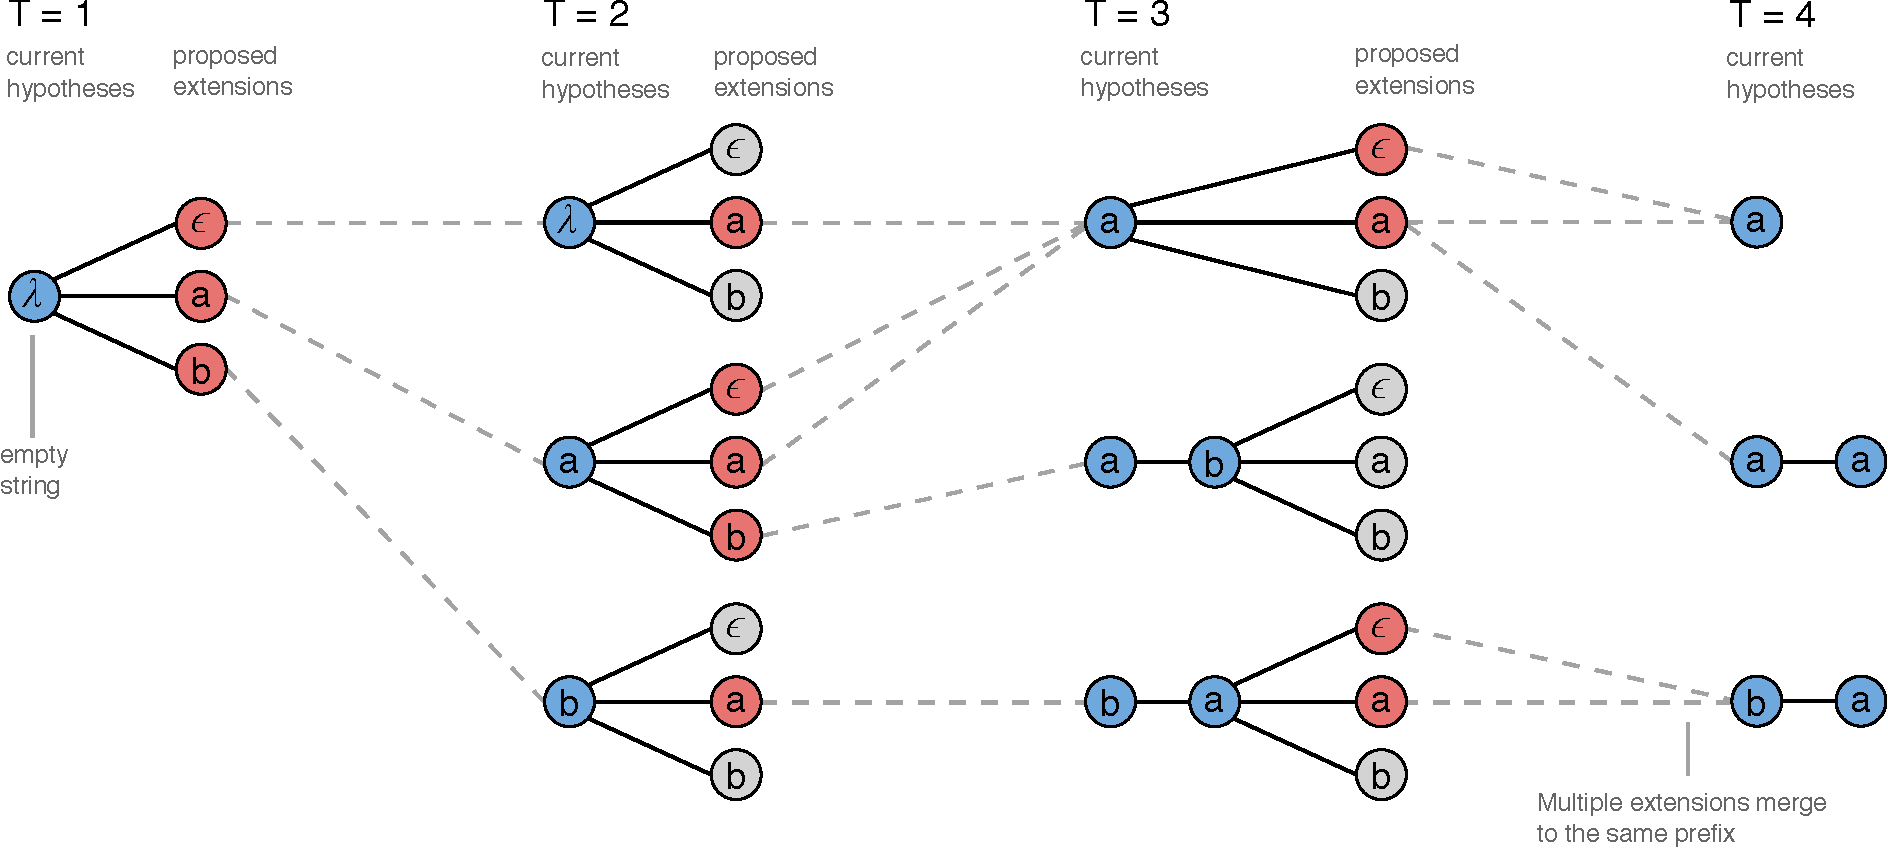
\includegraphics[width=\textwidth]{background/figures/prefix_beam_search.pdf}
\caption{The CTC beam search algorithm with an output alphabet $\{\epsilon, a,
    b\}$ and a beam size of three.}
\end{figure}

A proposed extension can map to two output prefixes if the character is a
repeat. This is shown at $T=3$ in the figure above where `a’ is proposed as an
extension to the prefix [a]. Both [a] and [a, a] are valid outputs for this
proposed extension.

When we extend [a] to produce [a, a], we only want include the part of the
previous score for alignments which end in $\epsilon$. Remember, the $\epsilon$
is required between repeat characters. Similarly, when we do not extend the
prefix and produce [a], we should only include the part of the previous score
for alignments which do not end in $\epsilon$.

Given this, we have to keep track of two probabilities for each prefix in the
beam. The probability of all alignments which end in $\epsilon$ and the
probability of all alignments which do not end in $\epsilon$. When we rank the
hypotheses at each step before pruning the beam, we will use their combined
scores.

The implementation of this algorithm does not require much code, but it is
dense and tricky to get right. See Algorithm~\ref{alg:background:decoder} for a
more rigorous description.

%% TODO, include algorithm here.

In some problems, such as speech recognition, incorporating a language model
over the outputs significantly improves accuracy. We can include the language
model as a factor in the inference problem.
\begin{align*}
Y^* \enspace = \enspace \argmax_Y \enspace
        p(Y \mid X) \cdot p(Y)^\alpha \cdot L(Y)^\beta
\end{align*}
The terms are respectively the CTC conditional probability, the language model
probability and a ``word" insertion bonus.

The function $L(Y)$ computes the length of $Y$ in terms of the language model
tokens and acts as a word insertion bonus. With a word-based language model
$L(Y)$ counts the number of words in $Y$. If we use a character-based language
model then $L(Y)$ counts the number of characters in $Y$. The language model
scores are only included when a prefix is extended by a character (or word) and
not at every step of the algorithm. This causes the search to favor shorter
prefixes, as measured by $L(Y)$, since they do not include as many language
model updates. The word insertion bonus helps with this. The parameters
$\alpha$ and $\beta$ are usually set by cross-validation.

The language model scores and word insertion term can be included in the beam
search. Whenever we propose to extend a prefix by a character, we can include
the language model score for the new character given the prefix so far.

\subsection{Properties of CTC}

We mentioned a few important properties of CTC so far. Here we will go into
more depth on what these properties are and what trade-offs they offer.

\subsubsection{Conditional Independence}

One of the most commonly cited shortcomings of CTC is the conditional
independence assumption it makes. The model assumes that every output is
conditionally independent of the other outputs given the input. This is a bad
assumption for many sequence to sequence problems.

Say we had an audio clip of someone saying ``triple A"~\cite{chan2016}. Another
valid transcription could be ``AAA". If the first letter of the predicted
transcription is `A', then the next letter should be `A' with high probability
and `r' with low probability. The conditional independence assumption does not
allow for this.

In fact speech recognizers using CTC do not learn a language model over the
output nearly as well as models which are conditionally
dependent~\cite{battenberg2017}. However, a separate language model can be
included and usually gives a good boost to accuracy.

The conditional independence assumption made by CTC is not always a bad thing.
Baking in strong beliefs over output interactions makes the model less
adaptable to new or altered domains. For example, we might want to use a speech
recognizer trained on phone conversations between friends to transcribe
customer support calls. The language in the two domains can be quite different
even if the acoustic model is similar. With a CTC acoustic model, we can easily
swap in a new language model as we change domains.

\subsubsection{Alignment Properties}

The CTC algorithm is {\it alignment-free}. The objective function marginalizes
over all alignments. While CTC does make strong assumptions about the form of
alignments between $X$ and $Y$, the model is agnostic as to how probability is
distributed amongst them. In some problems CTC ends up allocating most of the
probability to a single alignment. However, this is not guaranteed.\footnote{We
could force the model to choose a single alignment by replacing the sum with a
max in the objective function,
\[
p(Y \mid X) \enspace = \enspace \max_{A \in \mathcal{A}_{X,Y}} \enspace \prod_{t=1}^T \; p(a_t \mid X).
\]
}

As mentioned before, CTC only allows {\it monotonic} alignments. In problems
such as speech recognition this may be a valid assumption. For other problems
like machine translation where a future word in a target sentence can align to
an earlier part of the source sentence, this assumption is a deal-breaker.

Another important property of CTC alignments is that they are {\it
many-to-one}. Multiple inputs can align to at most one output. In some cases
this may not be desirable. We might want to enforce a strict one-to-one
correspondence between elements of $X$ and $Y$. Alternatively, we may want to
allow multiple output elements to align to a single input element. For example,
the characters ``th" might align to a single input step of audio. A character
based CTC model would not allow that.

The many-to-one property implies that the output cannot have more time-steps
than the input.\footnote{If $Y$ has $r$ consecutive repeats, then the length of
$Y$ must be less than the length of $X$ by $2r - 1$.} This is usually not a
problem for speech and handwriting recognition since the input is much longer
than the output. However, for other problems where $Y$ is often longer than
$X$, CTC will not work.

\subsection{CTC In Context}

In this section we will discuss how CTC relates to other commonly used
algorithms for sequence modeling.

\subsubsection{HMMs}

At a first glance, a Hidden Markov Model (HMM) seems quite different from
CTC. But, the two algorithms are actually quite similar. Understanding the
relationship between them will help us understand what advantages CTC has over
HMM sequence models and give us insight into how CTC could be changed for
various use cases.

Using the same notation as before, let $X$ be the input sequence and $Y$ be the
output sequence with lengths $T$ and $U$ respectively. We are interested in
learning $p(Y \mid X)$. One way to simplify the problem is to apply Bayes'
Rule:
\[
p(Y \mid X) \; \propto \; p(X \mid Y) \; p(Y).
\]

The $p(Y)$ term can be any language model, so let us focus on $p(X \mid Y)$.
Like before we will let $\mathcal{A}$ be a set of allowed of alignments between
$X$ and $Y$. Members of $\mathcal{A}$ have length $T$. Let us otherwise leave
$\mathcal{A}$ unspecified for now; we will come back to it later. We can
marginalize over alignments to get
\[
p(X \mid Y)\; = \; \sum_{A \in \mathcal{A}} \; p(X, A \mid Y).
\]
To simplify notation, we remove the conditioning on $Y$, it will be present in
every $p(\cdot)$. With two assumptions we can write down the standard HMM.
\begin{align*}
p(X) \enspace = \enspace \sum_{A \in \mathcal{A}} \; \prod_{t=1}^T \enspace
                p(x_t \mid a_t) \cdot p(a_t \mid a_{t-1})
\end{align*}
The probability of the input marginalizes over alignments the emission
probability, $p(x_t \mid a_t)$, and the transition probability, $p(a_t \mid
a_{t-1})$. The first assumption is the usual Markov property. The state $a_t$
is conditionally independent of all historic states given the previous state
$a_{t-1}$. The second is that the observation $x_t$ is conditionally
independent of everything given the current state $a_t$.

\begin{figure}
\centering
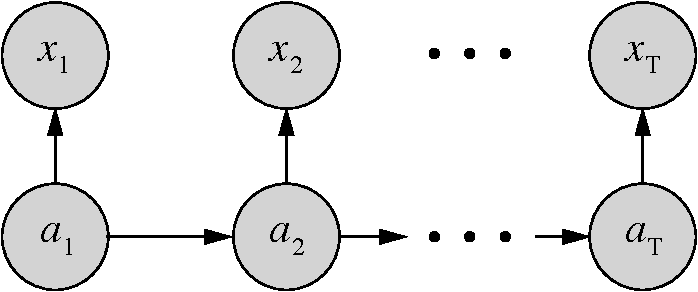
\includegraphics[width=0.4\textwidth]{background/figures/hmm.pdf}
\caption{The graphical model for an HMM.}
\end{figure}

Now we can take just a few steps to transform the HMM into CTC and see how
the two models relate. First, assume that the transition probabilities
$p(a_t \mid a_{t-1})$ are uniform. This gives
\[
p(X) \enspace \propto \enspace \sum_{A \in \mathcal{A}} \enspace \prod_{t=1}^T \; p(x_t \mid a_t).
\]
There are only two differences from this equation and the CTC loss function.
The first is that we are learning a model of $X$ given $Y$ as opposed to $Y$
given $X$. The second is how the set $\mathcal{A}$ is produced. We deal with
each in turn.

The HMM can be used with discriminative models which estimate $p(a \mid x)$.
To do this, we apply Bayes’ rule and rewrite the model as
\begin{align*}
p(X) \enspace &\propto \enspace \sum_{A \in \mathcal{A}} \enspace \prod_{t=1}^T \; \frac{p(a_t \mid x_t)\; p(x_t)}{p(a_t)} \\
    &\propto \enspace \sum_{A \in \mathcal{A}} \enspace \prod_{t=1}^T \; \frac{p(a_t \mid x_t)}{p(a_t)}.
\end{align*}

If we assume a uniform prior over the states $a$ and condition on all of $X$
instead of a single element at a time, we arrive at
\[
p(X) \enspace \propto \enspace \sum_{A \in \mathcal{A}} \enspace \prod_{t=1}^T \; p(a_t \mid X).
\]

The above equation is essentially the CTC loss function, assuming the set
$\mathcal{A}$ is the same. In fact, the HMM framework does not specify what
$\mathcal{A}$ should consist of. This part of the model can be designed on a
per-problem basis. In many cases the model does not condition on $Y$ and the
set $\mathcal{A}$ consists of all possible length $T$ sequences from the output
alphabet. In this case, the HMM can be drawn as an  {\it ergodic} state
transition diagram in which every state connects to every other state. The
figure below shows this model with the alphabet or set of unique hidden states
as $\{a, b, c\}$.

In our case the transitions allowed by the model are strongly related to $Y$.
We want the HMM to reflect this. One possible model could be a simple linear
state transition diagram. The figure below shows this with the same alphabet as
before and $Y =$ [a, b]. Another commonly used model is the {\it Bakis} or
left-right HMM. In this model any transition which proceeds from the left to
the right is allowed.

\begin{figure}
    \centering
    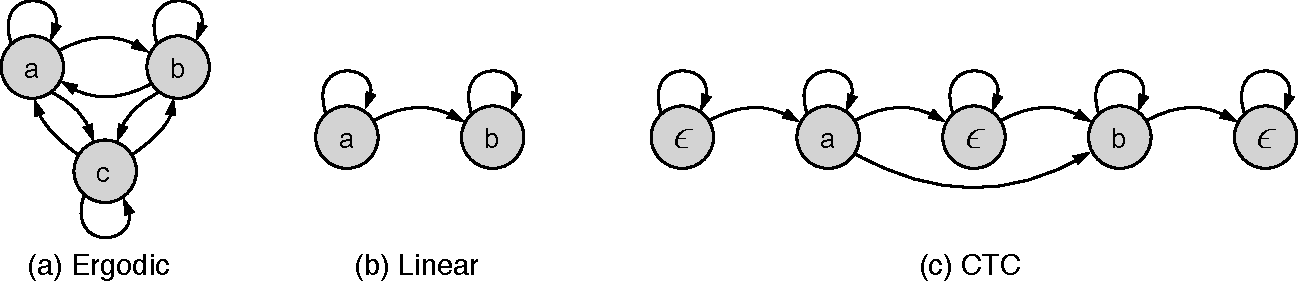
\includegraphics[width=\textwidth]{background/figures/hmm_types.pdf}
    \caption{Different HMM architectures.}
\end{figure}

In CTC we augment the alphabet with $\epsilon$ and the HMM model allows a
subset of the left-right transitions. The CTC HMM has two start states and two
accepting states.

One possible source of confusion is that the HMM model differs for any unique
$Y$. This is in fact standard in applications such as speech recognition. The
state diagram changes based on the output $Y$. However, the functions which
estimate the observation and transition probabilities are shared.

Let's discuss how CTC improves on the original HMM model. First, we can think
of the CTC state diagram as a special case HMM which works well for many
problems of interest. Incorporating the blank as a hidden state in the HMM
allows us to use the alphabet of $Y$ as the other hidden states. This model
also gives a set of allowed alignments which may be a good prior for some
problems.

Perhaps most importantly, CTC is discriminative. It models $p(Y \mid X)$
directly, an idea that has been important in the past with other discriminative
improvements to HMMs~\cite{woodland2002}.  Discriminative training allows us to
apply powerful learning algorithms like the RNN directly towards solving the
problem we care about.

\subsubsection{Encoder-Decoder Models}

The encoder-decoder is perhaps the most commonly used framework for sequence
modeling with neural networks. These models have an encoder and a decoder. The
encoder maps the input sequence $X$ into a hidden representation. The decoder
consumes the hidden representation and produces a distribution over the
outputs. We can write this as
\begin{align*}
H\enspace &= \enspace\textsf{encode}(X) \\[.5em]
p(Y \mid X)\enspace &= \enspace \textsf{decode}(H).
\end{align*}
The $\textsf{encode}(\cdot)$ and $\textsf{decode}(\cdot)$ functions are
typically RNNs. The decoder can optionally be equipped with an attention
mechanism. The hidden state sequence $H$ has the same number of time-steps as
the input, $T$. Sometimes the encoder subsamples the input. If the encoder
subsamples the input by a factor $s$ then $H$ will have $T/s$ time-steps.

We can interpret CTC in the encoder-decoder framework. This is helpful to
understand the developments in encoder-decoder models that are applicable to
CTC and to develop a common language for the properties of these models.

{\bf Encoder:} The encoder of a CTC model can be just about any encoder we find
in commonly used encoder-decoder models. For example the encoder could be a
multi-layer bidirectional RNN or a convolutional network. There is a constraint
on the CTC encoder that does not apply to the others. The input length cannot
be sub-sampled so much that $T/s$ is less than the length of the output.

{\bf Decoder:} We can view the decoder of a CTC model as a simple linear
transformation followed by a softmax normalization. This layer should project
all $T$ steps of the encoder output $H$ into the dimensionality of the output
alphabet.

We mentioned earlier that CTC makes a conditional independence assumption over
the characters in the output sequence. This is one of the big advantages that
other encoder-decoder models have over CTC -- they can model the dependence
over the outputs. However in practice, CTC is still more commonly used in tasks
like speech recognition as we can partially overcome the conditional
independence assumption by including an external language model.

\subsection{Practitioner's Guide}

So far we have mostly developed a conceptual understanding of CTC. Here we will
go through a few implementation tips for practitioners.

{\bf Software:} Even with a solid understanding of CTC, the implementation is
difficult. The algorithm has several edge cases and a fast implementation
should be written in a lower-level programming language.  Open-source software
tools make it much easier to get started:

\begin{itemize}
\item Baidu Research has open-sourced
    \texttt{warp-ctc}\footnote{https://github.com/baidu-research/warp-ctc}. The
    package is written in \C++ and CUDA. The CTC loss function runs on
    either the CPU or the GPU. Bindings are available for Torch, TensorFlow
    and PyTorch.
\item TensorFlow has built in CTC loss and beam search functions for the
    CPU.\footnote{https://www.tensorflow.org/api\_docs/python/tf/nn}
\item Nvidia also provides a GPU implementation of CTC in cuDNN versions 7 and
    up.\footnote{https://developer.nvidia.com/cudnn}
\end{itemize}

{\bf Numerical Stability:} Computing the CTC loss naively is numerically
unstable. One method to avoid this is to normalize the $\alpha$’s at each
time-step. The original publication has more detail on this including the
adjustments to the gradient~\cite{graves2006}. In practice this works well
enough for medium length sequences but can still underflow for long sequences.
A better solution is to compute the loss function in log-space with the
log-sum-exp trick.\footnote{When computing the sum of two probabilities in log
space use the identity
\[
\log(e^a + e^b) = \max\{a, b\} + \log(1 + e^{-|a-b|})
\]
Most programming languages have a stable function to compute $\log(1 + x)$ when
$x$ is close to zero.}

Inference should also be done in log-space using the log-sum-exp trick.

{\bf Beam Search:} There are a couple of good tips to know about when
implementing and using the CTC beam search.

The correctness of the beam search can be tested as follows.
\begin{enumerate}
\item Run the beam search algorithm on an arbitrary input.
\item Save the inferred output $\bar{Y}$ and the corresponding score $\bar{c}$.
\item Compute the actual CTC score $c$ for $\bar{Y}$.
\item Check that $\bar{c} \approx c$ with the former being no greater than the
      later. As the beam size increases the inferred output $\bar{Y}$ may change,
      but the two numbers should grow closer.
\end{enumerate}

A common question when using a beam search decoder is the size of the beam to
use. There is a trade-off between accuracy and runtime. We can check if the
beam size is in a good range. To do this first compute the CTC score for the
inferred output $c_i$. Then compute the CTC score for the ground truth output
$c_g$. If the two outputs are not the same, we should have $c_g < c_i$. If $c_i
<< c_g$ then the ground truth output actually has a higher probability under
the model and the beam search failed to find it. In this case a large increase
to the beam size may be warranted.
